\documentclass[10pt,a4paper]{article}

%%%%%%%%%%%%%%%%%%%%%%%%%%%%%%%%%%%%%%%%%%%%%%%%%%%%%%%%%%%%%%%%%%%%%%%%%%%%%%%%
% ENCODING

% Use UTF-8 as encoding
\usepackage[utf8]{inputenc}

%%%%%%%%%%%%%%%%%%%%%%%%%%%%%%%%%%%%%%%%%%%%%%%%%%%%%%%%%%%%%%%%%%%%%%%%%%%%%%%%
% LOGIC

% provides \isempty test
\usepackage{xstring, xifthen}

%%%%%%%%%%%%%%%%%%%%%%%%%%%%%%%%%%%%%%%%%%%%%%%%%%%%%%%%%%%%%%%%%%%%%%%%%%%%%%%%
% FONT

% Use Helvetica as main font
\usepackage[scaled]{helvet}

% Set font default
\renewcommand*\familydefault{\sfdefault}
\usepackage[T1]{fontenc}

% More font size definitions
\usepackage{moresize}

%%%%%%%%%%%%%%%%%%%%%%%%%%%%%%%%%%%%%%%%%%%%%%%%%%%%%%%%%%%%%%%%%%%%%%%%%%%%%%%%
% FONT AWESOME ICONS

% include the fontawesome icon set
\usepackage{fontawesome}

% use to vertically center content
% credits to: http://tex.stackexchange.com/questions/7219/how-to-vertically-center-two-images-next-to-each-other
\newcommand{\vcenteredinclude}[1]{\begingroup
\setbox0=\hbox{\includegraphics{#1}}%
\parbox{\wd0}{\box0}\endgroup}

% use to vertically center content
% credits to: http://tex.stackexchange.com/questions/7219/how-to-vertically-center-two-images-next-to-each-other
\newcommand*{\vcenteredhbox}[1]{\begingroup
\setbox0=\hbox{#1}\parbox{\wd0}{\box0}\endgroup}

% icon shortcut
\newcommand{\icon}[3] {
    \makebox(#2, #2){\textcolor{primary}{\csname fa#1\endcsname}}
}

% icon with text shortcut
\newcommand{\icontext}[4]{
    \vcenteredhbox{\icon{#1}{#2}{#3}}  \hspace{2pt}  \parbox{0.9\mpwidth}{\textcolor{#4}{#3}}
}

% icon with website url
\newcommand{\iconhref}[5]{
    \vcenteredhbox{\icon{#1}{#2}{#5}}  \hspace{2pt} \href{#4}{\textcolor{#5}{#3}}
}

% icon with email link
\newcommand{\iconemail}[5]{
    \vcenteredhbox{\icon{#1}{#2}{#5}}  \hspace{2pt} \href{mailto:#4}{\textcolor{#5}{#3}}
}

%%%%%%%%%%%%%%%%%%%%%%%%%%%%%%%%%%%%%%%%%%%%%%%%%%%%%%%%%%%%%%%%%%%%%%%%%%%%%%%%
% PAGE LAYOUT

% page outer frames (debug-only)
% \usepackage{showframe}

% Use paracol for 2-columns layout
\usepackage{paracol}

% Use A4 geometry
\usepackage[a4paper]{geometry}

% Remove all possible margins
\geometry{top=1cm, bottom=1cm, left=1cm, right=1cm}

\usepackage{fancyhdr}
\pagestyle{empty}

\setlength{\parindent}{0mm}

%%%%%%%%%%%%%%%%%%%%%%%%%%%%%%%%%%%%%%%%%%%%%%%%%%%%%%%%%%%%%%%%%%%%%%%%%%%%%%%%
% TABLE & ARRAY DEFINITIONS

% extended aligning of tabular cells
\usepackage{array}

% custom column right-align with fixed width
% use like p{size} but via x{size}
\newcolumntype{x}[1]{%
>{\raggedleft\hspace{0pt}}p{#1}}%

%%%%%%%%%%%%%%%%%%%%%%%%%%%%%%%%%%%%%%%%%%%%%%%%%%%%%%%%%%%%%%%%%%%%%%%%%%%%%%%%
% GRAPHICS DEFINITIONS

\usepackage{graphicx}
\usepackage{tikz}

%%%%%%%%%%%%%%%%%%%%%%%%%%%%%%%%%%%%%%%%%%%%%%%%%%%%%%%%%%%%%%%%%%%%%%%%%%%%%%%%
% COLORS

% Define some colors
\usepackage{transparent}
\usepackage{color}

% Primary color
\definecolor{primary}{RGB}{0,0,0}

% Light color
\definecolor{light}{RGB}{245,245,245}

%%%%%%%%%%%%%%%%%%%%%%%%%%%%%%%%%%%%%%%%%%%%%%%%%%%%%%%%%%%%%%%%%%%%%%%%%%%%%%%%
% LINKS

% Package for links, must be the last package used
\usepackage[hidelinks]{hyperref}

%%%%%%%%%%%%%%%%%%%%%%%%%%%%%%%%%%%%%%%%%%%%%%%%%%%%%%%%%%%%%%%%%%%%%%%%%%%%%%%%
% \mpwidth
%   Returns minipage width minus two times \fboxsep
%   width calculations. Can also be used for other boxes / environments
\newcommand{\mpwidth}{\linewidth-\fboxsep-\fboxsep}

%%%%%%%%%%%%%%%%%%%%%%%%%%%%%%%%%%%%%%%%%%%%%%%%%%%%%%%%%%%%%%%%%%%%%%%%%%%%%%%%
% \cvlist
%   Renders a standard LaTeX list but abstracts away the environment definition
\newcommand{\cvlist}[1] {
    \begin{itemize}{#1}\end{itemize}
}

%%%%%%%%%%%%%%%%%%%%%%%%%%%%%%%%%%%%%%%%%%%%%%%%%%%%%%%%%%%%%%%%%%%%%%%%%%%%%%%%
% \cvtext
\newcommand{\cvtext}[1] {
    \begin{tabular*}{1\mpwidth}{p{0.98\mpwidth}}
        \parbox{1\mpwidth}{#1}
    \end{tabular*}
}

%%%%%%%%%%%%%%%%%%%%%%%%%%%%%%%%%%%%%%%%%%%%%%%%%%%%%%%%%%%%%%%%%%%%%%%%%%%%%%%%
% \cvsection
\newcommand{\cvsection}[1] {
    \vspace{14pt}
    \cvtext{
        \textbf{\LARGE{\textcolor{primary}{\uppercase{#1}}}} \\[-4pt]
        \textcolor{primary}{\rule{\linewidth}{2pt}} \\
    }
}

%%%%%%%%%%%%%%%%%%%%%%%%%%%%%%%%%%%%%%%%%%%%%%%%%%%%%%%%%%%%%%%%%%%%%%%%%%%%%%%%
% \cvevent
% Renders a table and a paragraph (cvtext) wrapped in a parbox (to ensure minimum content
% is glued together when a pagebreak appears).
% Additional Information can be passed in text or list form (or other environments).
% the work you did
% param 1: time-frame i.e. Sep 14 - Jan 15 etc.
% param 2: event name (job position etc.)
% param 3: Customer, Employer, Industry
% param 4: Short description
% param 5: work done (optional)
% param 6: technologies include (optional)
% param 7: achievements (optional)
\newcommand{\cvevent}[7] {
    \parbox{\mpwidth}{
        \begin{tabular*}{1\mpwidth}{p{0.60\mpwidth} p{0.38\mpwidth}}
            \textcolor{black}{\textbf{#2}} & \hfill \textbf{#1} \\
        \end{tabular*}

        \cvtext{\textcolor{primary}{\textbf{#3}}}
        \vspace*{4pt}

        \ifthenelse{\isempty{#4}}{}{
            \cvtext{#4}\\
        }
    }

    \ifthenelse{\isempty{#5}}{}{
        {#5}
    }

    \ifthenelse{\isempty{#6}}{}{
        \cvtext{Technologies include:}\\
        {#6}
    }

    \ifthenelse{\isempty{#7}}{}{
        \cvtext{Achievements include:}\\[-12pt]
        {#7}
    }
    \vspace{14pt}
}

%%%%%%%%%%%%%%%%%%%%%%%%%%%%%%%%%%%%%%%%%%%%%%%%%%%%%%%%%%%%%%%%%%%%%%%%%%%%%%%%
% \cvproject
% Renders a table and a paragraph (cvtext) wrapped in a parbox (to ensure minimum content
% is glued together when a pagebreak appears).
% Additional Information can be passed in text or list form (or other environments).
% the work you did
% param 1: time-frame i.e. Sep 14 - Jan 15 etc.
% param 2: event name (job position etc.)
% param 3: Short description
\newcommand{\cvproject}[3] {
    \parbox{\mpwidth}{
        \begin{tabular*}{1\mpwidth}{p{0.60\mpwidth} p{0.38\mpwidth}}
            \textcolor{black}{\textbf{#2}} & \hfill \textbf{#1} \\
        \end{tabular*}

        \cvtext{#3} \\
    }

    \vspace{14pt}
}

\begin{document}
\columnratio{0.31}
\setlength{\columnsep}{2.2em}
\setlength{\columnseprule}{4pt}
\colseprulecolor{light}

\begin{paracol}{2}
\begin{leftcolumn}

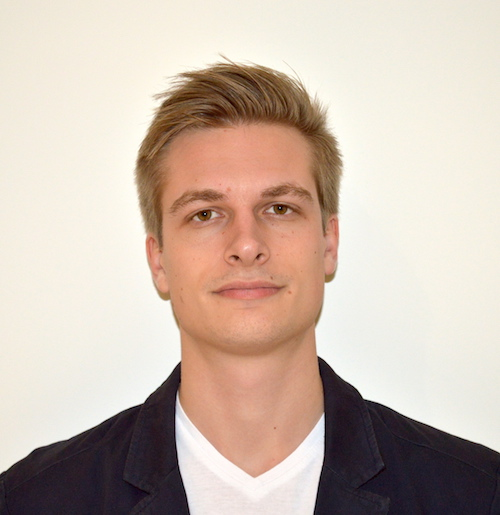
\includegraphics[width=\linewidth]{figures/photo.jpg}

%%%%%%%%%%%%%%%%%%%%%%%%%%%%%%%%%%%%%%%%%%%%%%%%%%%%%%%%%%%%%%%%%%%%%%%%%%%%%%%%
% CONTACT

\vspace{24pt}
\icontext{MapMarker}{12}{Lausanne, Switzerland}{black} \\

\vspace{-12pt}
\icontext{At}{12}{\href{mailto:lucas@elisei.ch}{lucas@elisei.ch}}{black} \\

\vspace{-12pt}
\icontext{Phone}{12}{On request}{black} \\

\vspace{-12pt}
\icontext{Globe}{12}{\href{https://elisei.ch}{elisei.ch}}{black} \\

\vspace{-12pt}
\icontext{Github}{12}{\href{https://github.com/faku99}{faku99}}{black} \\

%%%%%%%%%%%%%%%%%%%%%%%%%%%%%%%%%%%%%%%%%%%%%%%%%%%%%%%%%%%%%%%%%%%%%%%%%%%%%%%%
% LANGUAGES
\vfill
\cvsection{LANGUAGES}

\vspace{-12pt}
\cvtext{
\cvlist{
    \item French -- C2
    \item English -- C1
    \item Italian -- C2
}
}

%%%%%%%%%%%%%%%%%%%%%%%%%%%%%%%%%%%%%%%%%%%%%%%%%%%%%%%%%%%%%%%%%%%%%%%%%%%%%%%%
% SKILLS
\vfill
\cvsection{SKILLS}

\vspace{-12pt}
\cvtext{
\cvlist{
    \item Software development (C, Python, Javascript, Zig)
    \item Real-time firmware development \\ (FreeRTOS, Zephyr)
    \item Linux kernel drivers development
    \item Software architecture
    \item Risk \& requirements
    \item Medical devices (ISO 13485, IEC 62304)
    \item FPGA (VHDL, Vivado)
    \item Git
}
}

\vfill
\cvsection{REFERENCES}

\cvtext{
    On request
}

\newpage
\cvsection{INTERESTS}

\vspace{-12pt}
\cvtext{
\cvlist{
    \item Open-source projects
    \item Cycling
    \item Skiing
    \item Books
    \item Video games
    \item Traveling
}
}

%%%%%%%%%%%%%%%%%%%%%%%%%%%%%%%%%%%%%%%%%%%%%%%%%%%%%%%%%%%%%%%%%%%%%%%%%%%%%%%%
% BLOG POSTS
\vspace{20pt}
\cvsection{BLOG POSTS}

\vspace{-12pt}
\cvtext{
\cvlist{
    \item \href{https://blog.reds.ch/?p=1308}{A guide to compile and install a Xenomai-patched kernel}
}
}


\end{leftcolumn}
\begin{rightcolumn}

%%%%%%%%%%%%%%%%%%%%%%%%%%%%%%%%%%%%%%%%%%%%%%%%%%%%%%%%%%%%%%%%%%%%%%%%%%%%%%%%
% HEADER
\fcolorbox{white}{white}{\begin{minipage}[c][2cm][c]{1\mpwidth}
    \begin {center}
        \HUGE{ \textbf{ \textcolor{black}{ \uppercase{ LUCAS ELISEI } } } } \\[-24pt]
        \textcolor{black}{ \rule{0.1\textwidth}{1.25pt} } \\[4pt]
        \large{ \textcolor{black} {Senior Embedded Systems \& Firmware Engineer} }
    \end {center}
\end{minipage}} \\

%%%%%%%%%%%%%%%%%%%%%%%%%%%%%%%%%%%%%%%%%%%%%%%%%%%%%%%%%%%%%%%%%%%%%%%%%%%%%%%%
% PROFILE
\vfill\null
\cvsection{PROFILE}

\cvtext{
    Highly-motivated embedded systems engineer with five years of comprehensive experience, specializing in firmware
    development and architecture for medical devices. Proven track record in developing robust firmware solutions and
    leading technical initiatives within IEC 62304 and ISO 13485 regulated environments. Combines analytical thinking
    with interdisciplinary expertise to implement innovative solutions that improve people's lives through
    state-of-the-art technologies. \\
    Seeking new professional challenges to contribute technical leadership and firmware architecture expertise to dynamic medical device projects.
}

%%%%%%%%%%%%%%%%%%%%%%%%%%%%%%%%%%%%%%%%%%%%%%%%%%%%%%%%%%%%%%%%%%%%%%%%%%%%%%%%
% WORK EXPERIENCE
\vfill\null
\cvsection{WORK EXPERIENCE}

\cvevent
    {Sept 2022 - Present}
    {Firmware Engineer}
    {Tandem Diabetes Care Switzerland, Saint-Sulpice}
    {Developed the firmware for Sigi, an insulin patch pump in an IEC 62304 and ISO 13485 regulated environment.
    Project involved safety-critical architecture, using multiple MCUs and control loops.}
    {\cvtext{\cvlist{
        \item Was responsible of and developed safety-critical firmware modules
        \item Maintained Software Architecture, Design Specifications and other software documentation
        \item Defined backlog and led development of various features (System Base, Therapy Control and Hardware Control)
        \item Partnered closely with other teams to successfully bring the project forward
        \item Successfully led a development team as well as external contractors using SAFe methodology
    }}}
    {\cvtext{\cvlist{
        \item C, Python, Javascript
        \item FreeRTOS, Zephyr
        \item SAML21, Apollo3 Blue, STM32U5, nRF54
    }}}
    {}

\cvevent
    {March 2020 - June 2022}
    {Embedded Software Junior Developer}
    {REDS Institute, Yverdon-les-Bains}
    {Worked on various research projects (80\%) while being a teaching assistant (20\%).}
    {\cvtext{\cvlist{
        \item C/C++ user-space applications
        \item Linux kernel-space drivers
        \item High workload and high sampling frequency applications
        \item SoC development
        \item FPGA interfacing
        \item Teaching assistant for Operating Systems, Real-Time Processing and High-Performance Computing courses
    }}}
    {}
    {}

%%%%%%%%%%%%%%%%%%%%%%%%%%%%%%%%%%%%%%%%%%%%%%%%%%%%%%%%%%%%%%%%%%%%%%%%%%%%%%%%
% PROJECTS

\cvsection{PROJECTS}

\cvproject
    {Professional}
    {Selftest\_QRNG}
    {Self-testing Quantum Random Number Generator. High-workload project where data had to be passed to an embedded device and retrieve from it at rates around 200 Mbps. I was in charge of the whole software part, from hardware integration to kernel-space modules and user-space applications development.}

\cvproject
    {Professional}
    {HARE}
    {C framework that allows communication between actors in a publisher \& subscriber architecture. This framework had to handle considerable amount of incoming data (up to 40 Gbps). Also had to put all the hardware in place for a distributed acquisition of signals, synchronized with sub-nanosecond accuracy.}

\cvproject
    {Professional}
    {SmartTank}
    {An embedded system for monitoring the health of an oxygen tank on a automotive vehicle. I was in charge of the whole software part, from hardware integration to kernel-space modules and user-space applications development.}

\cvproject
    {Personal}
    {\href{https://github.com/2find/stereo}{\textbf{Stereo}}}
    {Flutter library for playing music from a file.}

\cvproject
    {Personal}
    {\href{http://cydia.saurik.com/package/com.faku99.goodges/}{\textbf{Goodges}}}
    {iOS extension for jailbroken devices. Radically changes the way notification badges are displayed on the homescreen.}

%%%%%%%%%%%%%%%%%%%%%%%%%%%%%%%%%%%%%%%%%%%%%%%%%%%%%%%%%%%%%%%%%%%%%%%%%%%%%%%%
% EDUCATION

\cvsection{EDUCATION}

\cvevent
    {Sept 2018 - June 2020}
    {Master of Science in Engineering}
    {Embedded Systems, HES-SO, Lausanne}
    {Thesis: ``Automatic Generation of FPGA-based Accelerators''}
    {}
    {}
    {}

\cvproject
    {Feb 2019 - June 2019}
    {Semester project}
    {``FPGA-based Accelerator for Machine Learning Inference''}

\cvevent
    {Sept 2015 - July 2018}
    {Bachelor of Engineering}
    {Embedded Systems, HEIG-VD, Yverdon-les-Bains}
    {Thesis: ``Just-in-Time Recompilation and Optimization of Compiled Binaries''}
    {}
    {}
    {}

\cvevent
    {Sept 2013 - July 2015}
    {Propedeutics}
    {Swiss Federal Institute of Technology (EPFL), Lausanne}
    {}
    {}
    {}
    {}

\cvproject
    {June 2013}
    {Scientifical Baccalauréat}
    {Mathematics speciality, mention \textit{Bien} with physics taught in English.}

% This is to ensure column separator goes all the way down
\vspace{135pt}

\end{rightcolumn}
\end{paracol}

\end{document}
